%package list
%%%%%%%%%%%%%%%%%%%%%%%%%%%%%%%%%%%%%%%%%%%%%%%%%%
\documentclass{article}
\usepackage[top=3cm, bottom=3cm, outer=3cm, inner=3cm]{geometry}
\usepackage{multicol}
\usepackage{graphicx}                  %LINE 225 C1 Y C2
\usepackage{url}
%\usepackage{cite}
\usepackage{hyperref}
\usepackage{array}
%\usepackage{multicol}
\newcolumntype{x}[1]{>{\centering\arraybackslash\hspace{0pt}}p{#1}}
\usepackage{natbib}
\usepackage{pdfpages}
\usepackage{multirow}
\usepackage[normalem]{ulem}
\useunder{\uline}{\ul}{}
\usepackage{svg}
\usepackage{xcolor}
\usepackage{listings}
\lstdefinestyle{ascii-tree}{
    literate={├}{|}1 {─}{--}1 {└}{+}1 
  }
\lstset{basicstyle=\ttfamily,
  showstringspaces=false,
  commentstyle=\color{red},
  keywordstyle=\color{blue}
}
%\usepackage{booktabs}
\usepackage{caption}
\usepackage{subcaption}
\usepackage{float}
\usepackage{array}

\newcolumntype{M}[1]{>{\centering\arraybackslash}m{#1}}
\newcolumntype{N}{@{}m{0pt}@{}}


%%%%%%%%%%%%%%%%%%%%%%%%%%%%%%%%%%%%%%%%%%%%%%%%%%%%%%%%%%%%%%%%%%%%%%%%%%%%
%%%%%%%%%%%%%%%%%%%%%%%%%%%%%%%%%%%%%%%%%%%%%%%%%%%%%%%%%%%%%%%%%%%%%%%%%%%%
\newcommand{\itemEmail}{aquispearr@unsa.edu.pe}
\newcommand{\itemEmail}{pcaril@unsa.edu.pe}
\newcommand{\itemStudentA}{
Quispe Arratea Alexandra Raquel}   
\newcommand{\itemStudentB}{Cari Lipe Paul Andree}   %line 134
%line 134

\newcommand{\itemCourse}{Pweb - II}
\newcommand{\itemCourseCode}{20212722}
\newcommand{\itemSemester}{I}
\newcommand{\itemUniversity}{Universidad Nacional de San Agustín de Arequipa}
\newcommand{\itemFaculty}{Facultad de Ingeniería de Producción y Servicios}
\newcommand{\itemDepartment}{Departamento Académico de Ingeniería de Sistemas e Informática}
\newcommand{\itemSchool}{Escuela Profesional de Ingeniería de Sistemas}
\newcommand{\itemAcademic}{2024 - A}
\newcommand{\itemInput}{Del 30 Abril 2024}
\newcommand{\itemOutput}{Al 4 Mayo 2024}
\newcommand{\itemPracticeNumber}{01}

%%%%%%%%%%%%%%%%%%%%%%%%%%%%%%%%%%%%%%%%%%%%%%%%%%%%%%%%%%%%%%%%%%%%%%%%%%%%
%%%%%%%%%%%%%%%%%%%%%%%%%%%%%%%%%%%%%%%%%%%%%%%%%%%%%%%%%%%%%%%%%%%%%%%%%%%%

\usepackage[english,spanish]{babel}
\usepackage[utf8]{inputenc}
\AtBeginDocument{\selectlanguage{spanish}}
\renewcommand{\figurename}{Figura}
\renewcommand{\refname}{Referencias}
\renewcommand{\tablename}{Tabla} 
\AtBeginDocument{%
	\renewcommand\tablename{Tabla}
}

\usepackage{fancyhdr}
\pagestyle{fancy}
\fancyhf{}
\setlength{\headheight}{30pt}
\renewcommand{\headrulewidth}{1pt}
\renewcommand{\footrulewidth}{1pt}
\fancyhead[L]{\raisebox{-0.2\height}{
\includegraphics[width=3cm]{img/logo_episunsa.png}}}
\fancyhead[C]{\fontsize{7}{7}\selectfont	\itemUniversity \\ \itemFaculty \\ \itemDepartment \\ \itemSchool \\ \textbf{\itemCourse}}
\fancyhead[R]{\raisebox{-0.2\height}{
\includegraphics[width=1.2cm]{img/logo_abet}}}
\fancyfoot[L]{Quispe Alexandra - Cari Paul}
\fancyfoot[C]{\itemCourse}
\fancyfoot[R]{Página \thepage}

% para el codigo fuente
\usepackage{listings}
\usepackage{color, colortbl}
\definecolor{dkgreen}{rgb}{0,0.6,0}
\definecolor{gray}{rgb}{0.5,0.5,0.5}
\definecolor{mauve}{rgb}{0.58,0,0.82}
\definecolor{codebackground}{rgb}{0.95, 0.95, 0.92}
\definecolor{tablebackground}{rgb}{0.8, 0, 0}

\lstset{frame=tb,
	language=bash,
	aboveskip=3mm,
	belowskip=3mm,
	showstringspaces=false,
	columns=flexible,
	basicstyle={\small\ttfamily},
	numbers=none,
	numberstyle=\tiny\color{gray},
	keywordstyle=\color{blue},
	commentstyle=\color{dkgreen},
	stringstyle=\color{mauve},
	breaklines=true,
	breakatwhitespace=true,
	tabsize=3,
	backgroundcolor= \color{codebackground},
}

\begin{document}
	
	\vspace*{10px}
	
	\begin{center}	
		\fontsize{17}{17} \textbf{Informe de Laboratorio  \itemPracticeNumber}
	\end{center}

	\begin{flushright}
		\begin{tabular}{|M{2.5cm}|N|}
			\hline 
			\rowcolor{tablebackground}
			\color{white} \textbf{Nota}  \\
			\hline 
			     \\[30pt]
			\hline 			
		\end{tabular}
	\end{flushright}	

	\begin{table}[H]
		\begin{tabular}{|x{4.7cm}|x{4.8cm}|x{4.8cm}|}
			\hline                                       %line 41
			\rowcolor{tablebackground}
			\color{white} \textbf{Estudiante} & \color{white}\textbf{Escuela}  & \color{white}\textbf{Asignatura}   \\
			\hline 
			{ \itemStudentA \par \itemStudentB \par \itemStudentC \par \itemStudentD \par\itemStudentE} &
			\itemSchool & {\itemCourse \par Semestre: \itemSemester}     \\
			\hline 			
		\end{tabular}
	\end{table}		
	
	\begin{table}[H]
		\begin{tabular}{|x{4.7cm}|x{4.8cm}|x{4.8cm}|}
			\hline 
			\rowcolor{tablebackground}
			\color{white}\textbf{Laboratorio} & \color{white}\textbf{Tema}  & \color{white}\textbf{Duración}   \\
			\hline 
			\itemPracticeNumber & \itemTheme & 24 horas aprox.\\
			\hline 
		\end{tabular}
	\end{table}
	
	\begin{table}[H]
		\begin{tabular}{|x{4.7cm}|x{4.8cm}|x{4.8cm}|}
			\hline 
			\rowcolor{tablebackground}
			\color{white}\textbf{Semestre académico} & \color{white}\textbf{Fecha de inicio}  & \color{white}\textbf{Fecha de entrega}   \\
			\hline 
			\itemAcademic & \itemInput &  \itemOutput  \\
			\hline 
		\end{tabular}
	\end{table}
	
	\section{Tarea}
	\begin{itemize}		%line 200 first commit
		\item \textbf{}
Crear un contenedor en Docker basado en Ubuntu 20.04:
\begin{itemize}
    \item Especificaciones del Lab 01
    \begin{itemize}
        \item Instale el servidor web Apache HTTP server 2.x
        \item Instale cualquiera de estos lenguajes de programación: PHP, Perl, Python.
        \item Configure el servidor web para que interprete uno de los lenguajes de programación.
        \item Instale cualquiera de los servidores de base de datos: MySQL, MariaDB, PostgreSQL.
        \item Instale el servidor Open SSH Server. Envíe archivos al servidor: imágenes, CSS, JS, etc.
        \item Cree un usuario \texttt{pw2} con contraseña: \texttt{12345678}.
        \item Otorgue permisos al usuario para acceder a la aplicación web. (Read/Write)
        \item Finalmente, implemente el trabajo final del curso de \texttt{pw1} en ese contenedor.
        \item Elabore un informe paso a paso donde explique funcionalmente el proyecto, demostrando que se trata de un contenedor Docker.
        \item Adjunte la URL de un video donde muestre que se trata de un contenedor Docker.
    \end{itemize}
\end{itemize}
 

	\end{itemize}
		
	\section{Equipos, materiales y temas utilizados}
	\begin{itemize}
		\item Sistemas Operativos Ubuntu y Windows 
		\item NVIM v0.6.1, VSCode, Eclipse
		\item OpenJDK 64-Bits 11, 17, 18
		\item Git 2.34.1 y versiones posteriores
		\item Cuentas en GitHub/GitLab con el correo institucional.

	\end{itemize}
	
	\section{URL de Repositorio Github}
	\begin{itemize}
		\item URL del Repositorio GitHub para clonar o recuperar.
		\item \url{https://github.com/aquispearr/pweb2_lab01}
  \item URL del repositorio GitLab para clonar o recuperar.
  \item \url{https://gitlab.com/aquispearr/pweb2_lab01}
	\end{itemize}
	
	

%%%%%%%%%%%%%%%%%%%%%%%%%%%%%%%%%%%%%%%%%%%%%%%%%%%%%%%%%%%%%%%%%%%%%%%%%%%%%%%%%%%%%%%%%%%%%%%%%%%%%%%%%%%%%%%%%%%%%%%%%%%%%%%%%%%%%%%%%%%%%%%%%%%%%%%%%%%%%%%%%%%%%%%%%%%%%%%%%%%%%%%%%%%%%%%%%%%
\section{Proyecto Final de Pweb1}


&&&&&&&&&&&&&&&&&&&&&&&&&&&&&&&&&&&&&&&&&&&&&&&&&&&&&&&&&&&&&&&&&&&&&&&&&&&&&
\section{Desarrollo }
&&&&&&&&&&&&&&&&&&&&&&&&&&&&&&&&&&&&&&&&&&&&&&&&&&&&&&&&&&&&&&&&&&&&&&&&&&&&&
\subsection{Docker pull}

Paso 1: Descargar la imagen de Ubuntu

En este paso, descargamos la imagen de Ubuntu desde el repositorio de Docker Hub utilizando el comando \texttt{docker pull}.

\begin{figure}[h]
    \centering
    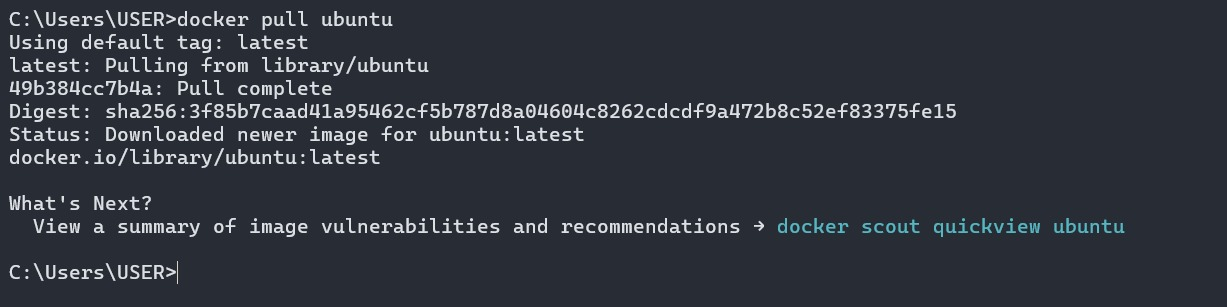
\includegraphics[width=1\textwidth]{latex/img/docker_pull.png}
    \caption{Proceso de descarga de la imagen de Ubuntu}
    \label{fig:docker_pull}
\end{figure}

En la captura de pantalla proporcionada, se puede observar el proceso de descarga de la imagen de Ubuntu. A continuación, se detallan los pasos realizados:




Es importante destacar que la imagen de Ubuntu descargada servirá como base para la creación de nuestro contenedor Docker, sobre el cual se llevará a cabo la instalación y configuración de los servicios requeridos para el laboratorio.


%%%%%%%%%%%%%%%%%%%%%%%%%%%%%%%%%%%%%%%%%%%%%%%%%%%%%%%%%%%%%%%%%%%%%%%%%%%
\subsection{Docker run}

En este paso, creamos un contenedor Docker a partir de la imagen de Ubuntu descargada anteriormente. Además, configuramos los puertos necesarios para la conexión a la base de datos y otros servicios requeridos según las especificaciones del laboratorio.

\begin{figure}[h]
    \centering
    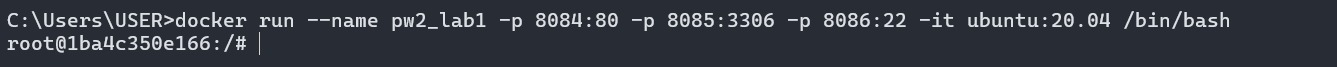
\includegraphics[width=1\textwidth]{latex/img/docker_run.png}
    \caption{Creación del contenedor Docker}
    \label{fig:docker_run}
\end{figure}

En la captura de pantalla proporcionada, se muestra el comando \texttt{docker run} utilizado para crear el contenedor Docker. A continuación, se detallan los parámetros utilizados y su función:

\begin{itemize}
    \item \textbf{Nombre del contenedor (\texttt{--name pw2\_labl}):} \\
    \begin{lstlisting}[language=bash]
    C:\Users\USER>docker run --name pw2_labl -p 8084:80 -p 8085:3306 -p 8086:22 -it ubuntu:20.04 /bin/bash
    \end{lstlisting}
    Especificamos el nombre del contenedor como "pw2\_labl" utilizando la opción \texttt{--name}. Este nombre será utilizado para hacer referencia al contenedor en operaciones posteriores.

    \item \textbf{Mapeo de puertos (\texttt{-p 8084:80 -p 8085:3306 -p 8086:22}):} \\
    Utilizamos la opción \texttt{-p} para mapear los puertos del contenedor a los puertos del host. En este caso, hemos mapeado los siguientes puertos:
    \begin{itemize}
        \item Puerto 80 del contenedor (utilizado por el servidor web) al puerto 8084 del host.
        \item Puerto 3306 del contenedor (utilizado por la base de datos) al puerto 8085 del host.
        \item Puerto 22 del contenedor (utilizado por SSH) al puerto 8086 del host.
    \end{itemize}

    \item \textbf{Interactividad y acceso a la terminal (\texttt{-it}):} \\
    Utilizamos las opciones \texttt{-it} para mantener el contenedor en modo interactivo y acceder a su terminal.

    \item \textbf{Imagen base (\texttt{ubuntu:20.04}):} \\
    Especificamos la imagen base a partir de la cual se creará el contenedor, que en este caso es Ubuntu 20.04.

    \item \textbf{Shell (\texttt{/bin/bash}):} \\
    Indicamos el shell que queremos utilizar una vez que el contenedor esté en funcionamiento, en este caso, Bash.
\end{itemize}


&&&&&&&&&&&&&&&&&&&&&&&&&&&&&&&&&&&&&&&&&&&&&&&&&&&&&&&&&&&&&&&&&&&&&&&&&&&&&
\subsection{Actualización del Sistema Operativo}

En este paso, realizamos una actualización de los repositorios del sistema operativo Ubuntu utilizando el comando \texttt{apt-get update}.

\begin{figure}[h]
    \centering
    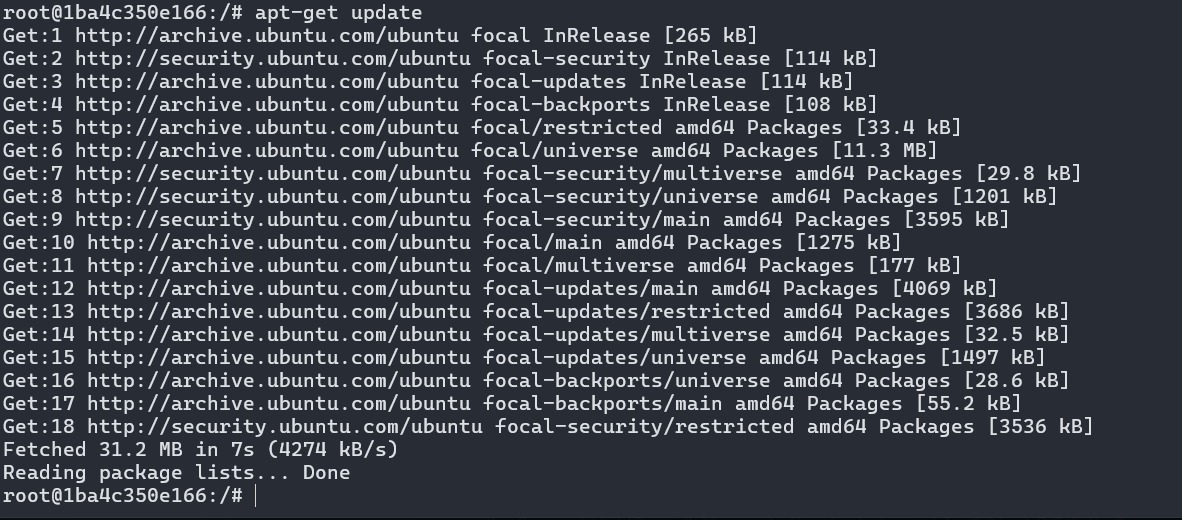
\includegraphics[width=1\textwidth]{latex/img/apt-get-update.png}
    \caption{Ejecución del comando \texttt{apt-get update}}
    \label{fig:apt-get-update}
\end{figure}

En la captura de pantalla proporcionada, se muestra la ejecución del comando \texttt{apt-get update}. A continuación, se detalla la salida relevante del comando:

\begin{itemize}
    \item \textbf{Descarga de actualizaciones de repositorios:} \\
    El comando \texttt{apt-get update} realiza la descarga de información sobre los paquetes disponibles en los repositorios configurados en el sistema operativo.
    \begin{lstlisting}[language=java]
    root@1ba4c350e166: /# apt-get update
    \end{lstlisting}

    \item \textbf{Progreso de actualización y lectura de listas de paquetes:} \\
    Se observa el progreso de la descarga de la información de los repositorios y una vez completada la descarga, se muestra el mensaje "Reading package lists... Done", indicando que el proceso ha finalizado satisfactoriamente.
\end{itemize}

Este paso es importante para asegurarnos de que nuestro sistema operativo tenga acceso a la información más reciente sobre los paquetes disponibles en los repositorios, lo cual es fundamental para la instalación de software adicional requerido para nuestro entorno de trabajo.


&&&&&&&&&&&&&&&&&&&&&&&&&&&&&&&&&&&&&&&&&&&&&&&&&&&&&&&&&&&&&&&&&&&&&&&&&&&&&
\subsection{Instalación del Editor de Texto Vim}

En este paso, instalamos el editor de texto Vim dentro del contenedor Docker. Vim es un editor de texto altamente configurable, que facilita la edición de archivos de configuración y código fuente.

\begin{figure}[h]
    \centering
    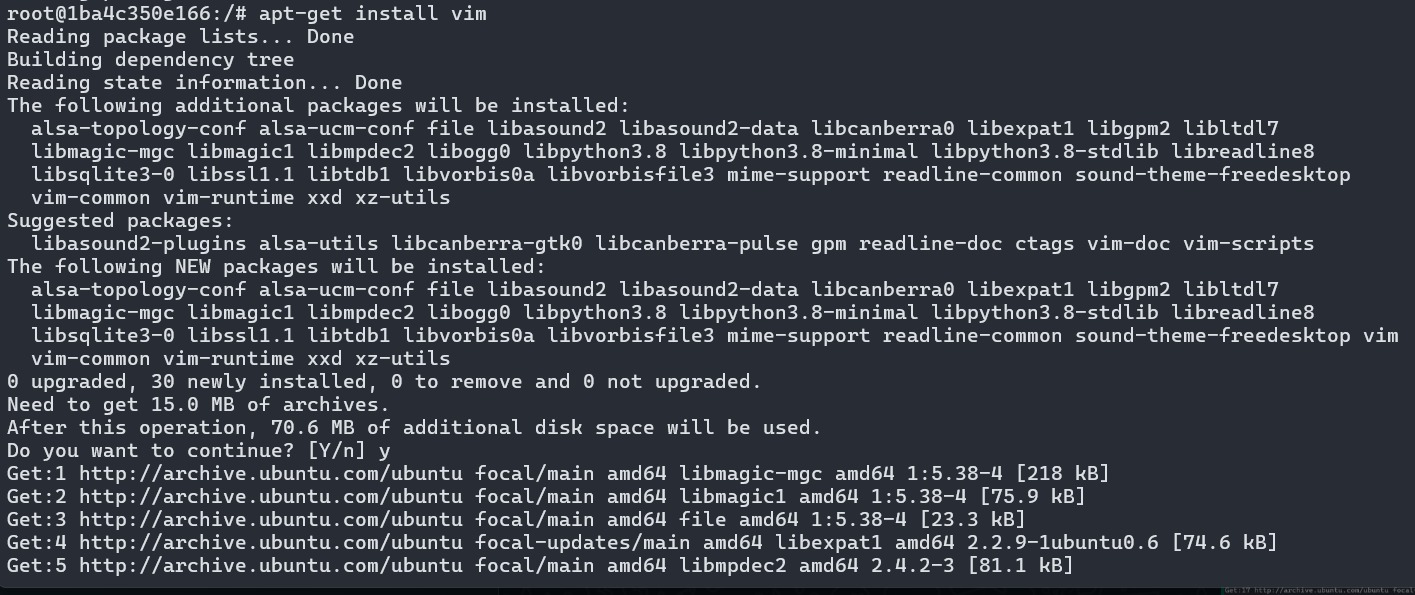
\includegraphics[width=1\textwidth]{latex/img/install_vim.jpeg}
    \caption{Ejecución del comando \texttt{apt-get install vim}}
    \label{fig:install_vim}
\end{figure}

En la captura de pantalla proporcionada, se muestra el comando \texttt{apt-get install vim} utilizado para instalar Vim dentro del contenedor Docker. A continuación, se detallan los pasos realizados y los detalles observados en la captura de pantalla:

\begin{itemize}
    \item \textbf{Ejecución del comando \texttt{apt-get install vim}:} \\
    Este comando se utiliza para iniciar el proceso de instalación del editor de texto Vim en el sistema operativo Ubuntu dentro del contenedor Docker.

    \item \textbf{Lectura de los paquetes a instalar:} \\
    La terminal muestra una lista de los paquetes adicionales que serán instalados junto con Vim, así como la cantidad de espacio en disco que se utilizará.

    \item \textbf{Confirmación de la instalación:} \\
    Se solicita confirmación para proceder con la instalación de los paquetes adicionales y la ocupación de espacio en disco.

    \item \textbf{Progreso de la instalación:} \\
    La terminal muestra el progreso de la descarga e instalación de los paquetes necesarios para Vim.
\end{itemize}

Una vez completada la instalación, Vim estará disponible en el sistema y listo para su uso. Este editor de texto será útil para la edición de archivos de configuración, código fuente y cualquier otro tipo de archivo de texto necesario durante el desarrollo y configuración del entorno de trabajo en el contenedor Docker.




&&&&&&&&&&&&&&&&&&&&&&&&&&&&&&&&&&&&&&&&&&&&&&&&&&&&&&&&&&&&&&&&&&&&&&&&&&&&&
\subsection{Instalación del Servidor MariaDB}

En este paso, instalamos el servidor MariaDB dentro del contenedor Docker. MariaDB es un sistema de gestión de bases de datos relacional que proporciona un reemplazo compatible con MySQL.

    \begin{lstlisting}[language=java]
    root@1ba4c350e166: /# apt-get install mariadb-server
    \end{lstlisting}


\begin{figure}[h]
    \centering
    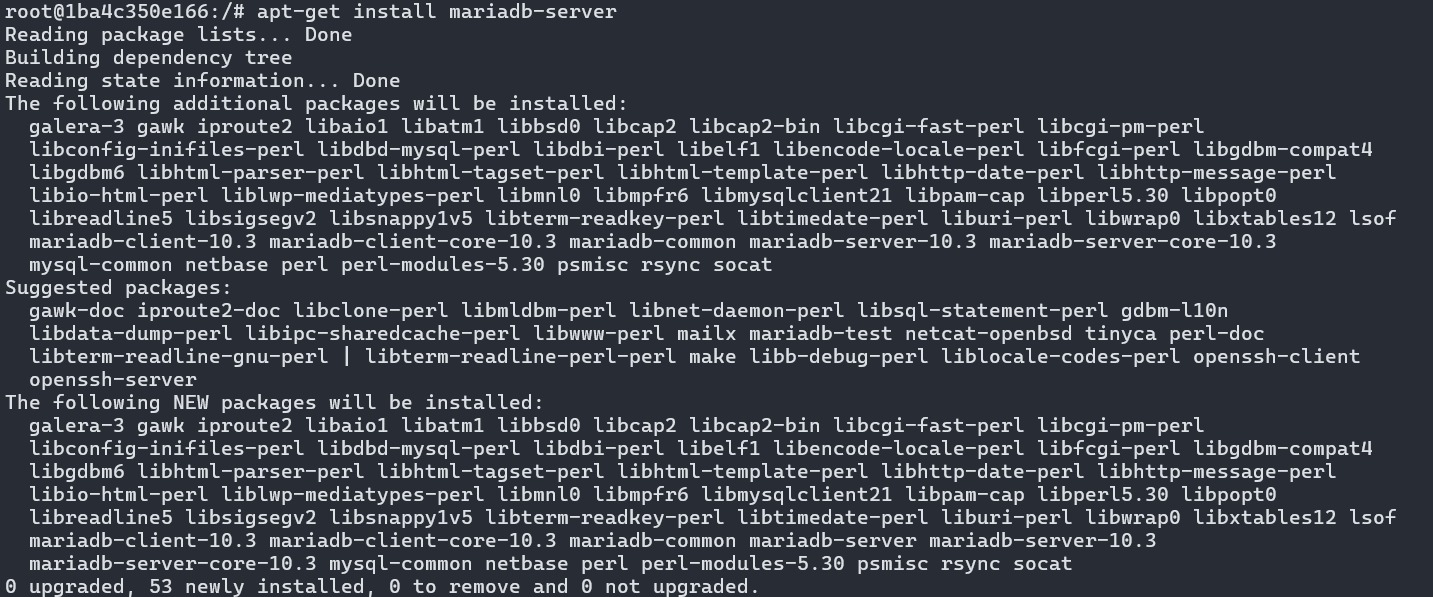
\includegraphics[width=1\textwidth]{latex/img/mariadb_server.png}
    \caption{Ejecución del comando \texttt{apt-get install mariadb-server}}
    \label{fig:mariadb_server}
\end{figure}

En la captura de pantalla proporcionada, se muestra el comando \texttt{apt-get install mariadb-server} utilizado para instalar el servidor MariaDB dentro del contenedor Docker. 

&&&&&&&&&&&&&&&&&&&&&&&&&&&&&&&&&&&&&&&&&&&&&&&&&&&&&&&&&&&&&&&&&&&&&&&&&&&&&

%%%%%%%%%%%%%%%%%%%%%%%%%%%%%%%%%%%%%%%%%%%%%%%%%%%%%%%%%%%%%%%%%%

\section{Instalación del Servidor Apache}

En este paso, instalamos el servidor Apache dentro del contenedor Docker. Apache es un servidor web ampliamente utilizado que permite alojar sitios web y servir contenido web estático y dinámico.

\begin{figure}[h]
    \centering
    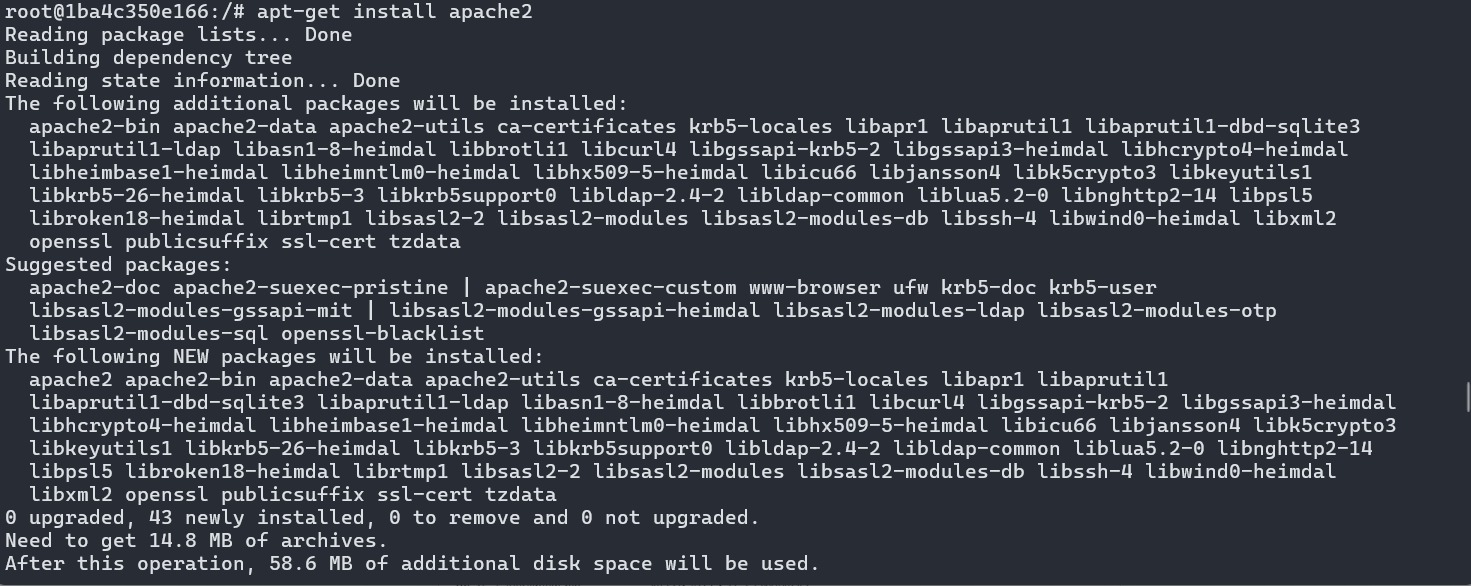
\includegraphics[width=1\textwidth]{latex/img/install_apache.png}
    \caption{Instalación del servidor Apache}
    \label{fig:install_apache}
\end{figure}

En la captura de pantalla proporcionada, se muestra el comando \texttt{apt-get install apache2} utilizado para instalar el servidor Apache dentro del contenedor Docker. A continuación, se detallan los pasos realizados y los detalles observados en la captura de pantalla:

\begin{itemize}
    \item \textbf{Ejecución del comando \texttt{apt-get install apache2}:} \\
    Este comando inicia el proceso de instalación del servidor Apache en el sistema operativo Ubuntu dentro del contenedor Docker.

    \item \textbf{Progreso de la instalación:} \\
    La terminal muestra el progreso de la descarga e instalación de los paquetes necesarios para Apache.

    \item \textbf{Confirmación de la instalación:} \\
    Se muestra un mensaje solicitando confirmación para proceder con la instalación de los paquetes adicionales y la ocupación de espacio en disco.

    \item \textbf{Finalización de la instalación:} \\
    Una vez completada la instalación, Apache estará disponible en el sistema y listo para servir contenido web.
\end{itemize}

Este paso es fundamental para configurar un entorno de desarrollo web dentro del contenedor Docker, donde podremos alojar y probar nuestros sitios y aplicaciones web de manera local.















%%%%%%%%%%%%%%%%%%%%%%%%%%%%%%%%%%%%%%%%%%%%%%%%%%%%%%%%%%%%%%%%%%%%%%%%%%%%%%%%%%%%%%%%%%%%%%%%%%%%%%%%%%%%%%%%%%%%%%%%%%%%%%%%%%%%%%%%%%%%%%%%%%%%%%%%%%%%%%%%%%%%%%%%%%%%%%%%%%%%%%%%%%%%%%%%%%%
	\section{\textcolor{red}{Rúbricas}}
	
	\subsection{\textcolor{red}{Entregable Informe}}
	\begin{table}[H]
		\caption{Tipo de Informe}
		\setlength{\tabcolsep}{0.5em} % for the horizontal padding
		{\renewcommand{\arraystretch}{1.5}% for the vertical padding
		\begin{tabular}{|p{3cm}|p{12cm}|}
			\hline
			\multicolumn{2}{|c|}{\textbf{\textcolor{red}{Informe}}}  \\
			\hline 
			\textbf{\textcolor{red}{Latex}} & \textcolor{blue}{El informe está en formato PDF desde Latex,  con un formato limpio (buena presentación) y facil de leer.}   \\ 
			\hline 
			
			
		\end{tabular}
	}
	\end{table}



	\subsection{\textcolor{red}{Rúbrica para el contenido del Informe y demostración}}
	\begin{itemize}			
		\item El alumno debe marcar o dejar en blanco en celdas de la columna \textbf{Checklist} si cumplio con el ítem correspondiente.
		\item Si un alumno supera la fecha de entrega,  su calificación será sobre la nota mínima aprobada, siempre y cuando cumpla con todos lo items.
		\item El alumno debe autocalificarse en la columna \textbf{Estudiante} de acuerdo a la siguiente tabla:
	
		\begin{table}[ht]
			\caption{Niveles de desempeño}
			\begin{center}
			\begin{tabular}{ccccc}
    			\hline
    			 & \multicolumn{4}{c}{Nivel}\\
    			\cline{1-5}
    			\textbf{Puntos} & Insatisfactorio 25\%& En Proceso 50\% & Satisfactorio 75\% & Sobresaliente 100\%\\
    			\textbf{2.0}&0.5&1.0&1.5&2.0\\
    			\textbf{4.0}&1.0&2.0&3.0&4.0\\
    		\hline
			\end{tabular}
		\end{center}
	\end{table}	
	
	\end{itemize}
	
	\begin{table}[H]
		\caption{Rúbrica para contenido del Informe y demostración}
		\setlength{\tabcolsep}{0.5em} % for the horizontal padding
		{\renewcommand{\arraystretch}{1.5}% for the vertical padding
		%\begin{center}
		\begin{tabular}{|p{2.7cm}|p{7cm}|x{1.3cm}|p{1.2cm}|p{1.5cm}|p{1.1cm}|}
			\hline
    		\multicolumn{2}{|c|}{Contenido y demostración} & Puntos & Checklist & Estudiante & Profesor\\
			\hline
			\textbf{1. GitHub} & Hay enlace URL activo del directorio para el  laboratorio hacia su repositorio GitHub con código fuente terminado y fácil de revisar. &2 &X &2 & \\ 
			\hline
			\textbf{2. Commits} &  Hay capturas de pantalla de los commits más importantes con sus explicaciones detalladas. (El profesor puede preguntar para refrendar calificación). &4 &X &3 & \\ 
			\hline 
			\textbf{3. Código fuente} &  Hay porciones de código fuente importantes con numeración y explicaciones detalladas de sus funciones. &2 &X &2 & \\ 
			\hline 
			\textbf{4. Ejecución} & Se incluyen ejecuciones/pruebas del código fuente  explicadas gradualmente. &2 &X &1 & \\ 
			\hline			
			\textbf{5. Pregunta} & Se responde con completitud a la pregunta formulada en la tarea.  (El profesor puede preguntar para refrendar calificación).  &2 &X &1 & \\ 
			\hline	
			\textbf{6. Fechas} & Las fechas de modificación del código fuente estan dentro de los plazos de fecha de entrega establecidos. &2 &X &2 & \\ 
			\hline 
			\textbf{7. Ortografía} & El documento no muestra errores ortográficos. &2 &X &2 & \\ 
			\hline 
			\textbf{8. Madurez} & El Informe muestra de manera general una evolución de la madurez del código fuente,  explicaciones puntuales pero precisas y un acabado impecable.   (El profesor puede preguntar para refrendar calificación).  &4 &X &3 & \\ 
			\hline
			\multicolumn{2}{|c|}{\textbf{Total}} &20 & &19 & \\ 
			\hline
		\end{tabular}
		%\end{center}
		%\label{tab:multicol}
		}
	\end{table}
	
\clearpage

\section{Referencias}
\begin{itemize}			
	\item \url{https://www.geeksforgeeks.org/insertion-sort/}
\end{itemize}	
	
%\clearpage
%\bibliographystyle{apalike}
%\bibliographystyle{IEEEtranN}
%\bibliography{bibliography}
			
\end{document}
